\documentclass{../../oss-apphys}
\usepackage{amssymb}
\usepackage{bm}

\begin{document}
\genheader

\gentitle{1 \& C}{DYNAMICS}{1 \& 2}

\genmultidirections

\gengravity

\raggedcolumns
\begin{multicols}{2}

  \begin{enumerate}[leftmargin=18pt]
    
%  \item A \SI{10}{\gram} penny is dropped from a building that is \SI{125}{m}
%    high. The penny is initially at rest. Approximately how long does it take
%    the penny to hit the ground?
%    \begin{enumerate}[noitemsep,topsep=0pt,leftmargin=18pt,label=(\Alph*)]
%    \item\SI{3.2}{\second}
%    \item\SI{4.5}{\second}
%    \item\SI{10}{\second}
%    \item\SI{15}{\second}
%    \item\SI{20}{\second}
%    \end{enumerate}
%
%  \item A car in a drag race started from rest and accelerated constantly to a
%    velocity of \SI{50}{m/s} when it reached the end of a \SI{500}{\metre} road.
%    What was the car's rate of acceleration?
%    \begin{enumerate}[noitemsep,topsep=0pt,leftmargin=18pt,label=(\Alph*)]
%    \item\SI{-5.0}{m/s^2}
%    \item\SI{-2.5}{m/s^2}
%    \item\SI{0.5 }{m/s^2}
%    \item\SI{2.5 }{m/s^2}
%    \item\SI{5.0 }{m/s^2}
%    \end{enumerate}
%  \end{enumerate}
%
%  \textbf{Questions 3 to 6}
%  The motion of the car is represented in the following graph.
%  
%  \columnbreak
%  \begin{enumerate}[leftmargin=18pt,resume]
%  \item Which of the following best describes the motion of the car in regions
%    C, D, and E of the velocity versus time graph?
%    \begin{enumerate}[noitemsep,topsep=0pt,leftmargin=18pt,label=(\Alph*)]
%    \item It is slowing down until in reverses direction and speeds back up
%      again.
%    \item It moves at a constant velocity in the negative direction.
%    \item It accelerates at a constant, nonzero acceleration except at point C
%      when its acceleration is zero.
%    \item Its position changes at a constant rate.
%    \item It moves at a constant, positive acceleration throughout the trip.
%    \end{enumerate}
%
%  \item What is the magnitude of the acceleration of the car in region A?
%    \begin{enumerate}[noitemsep,topsep=0pt,leftmargin=18pt,label=(\Alph*)]
%    \item\SI{0 }{m/s^2}
%    \item\SI{3 }{m/s^2}
%    \item\SI{5 }{m/s^2}
%    \item\SI{10}{m/s^2}
%    \item\SI{30}{m/s^2}
%    \end{enumerate}
%    
%  \item What is the acceleration rate of the car at the 6-second clock
%    reading?
%    \begin{enumerate}[noitemsep,topsep=0pt,leftmargin=18pt,label=(\Alph*)]
%    \item\SI{0  }{m/s^2}
%    \item\SI{-15}{m/s^2}
%    \item\SI{-30}{m/s^2}
%    \item\SI{+30}{m/s^2}
%    \item\SI{-60}{m/s^2}
%    \end{enumerate}
%    
%  \item Rank the average velocities of the car in regions A, B, C, and E.
%    \begin{enumerate}[noitemsep,topsep=0pt,leftmargin=18pt,label=(\Alph*)]
%    \item $A > B > C = E$
%    \item $B = A > C = E$
%    \item $B > A = C = E$
%    \item $B > A = C > E$
%    \item $A > B > C = E$
%    \end{enumerate}
%    
%  \item An airplane is flying horizontally at a velocity of \SI{50.0}{m/s} at an
%    altitude of \SI{125}{\metre}. It drops a package to observers on the ground
%    below. Approximately how far will the package travel in the horizontal
%    direction from the point that it was dropped?
%    \begin{enumerate}[noitemsep,topsep=0pt,leftmargin=18pt,label=(\Alph*)]
%    \item\SI{100}{\metre}
%    \item\SI{159}{\metre}
%    \item\SI{250}{\metre}
%    \item\SI{1020}{\metre}
%    \item\SI{1590}{\metre}
%    \end{enumerate}
%    
%  \item A placekicker kicks a football at a velocity of \SI{10.0}{m/s} from a
%    tee on the ground at an angle of \ang{30} from the horizontal.
%    Approximately how long will the ball stay in the air?
%    \begin{enumerate}[noitemsep,topsep=0pt,leftmargin=18pt,label=(\Alph*)]
%    \item\SI{0.0}{\second}
%    \item\SI{0.6}{\second}
%    \item\SI{0.8}{\second}
%    \item\SI{1.0}{\second}
%    \item\SI{1.8}{\second}
%    \end{enumerate}
%    
%  \item A car is traveling at an unknown velocity. It accelerates constantly
%    over \SI{5.0}{\second} at a rate of \SI{3.0}{m/s^2} to reach a velocity of
%    \SI{30}{m/s}. What was the original velocity of the car?
%    \begin{enumerate}[noitemsep,topsep=0pt,leftmargin=18pt,label=(\Alph*)]
%    \item\SI{1.0}{m/s}
%    \item\SI{5.0}{m/s}
%    \item\SI{10 }{m/s}
%    \item\SI{15 }{m/s}
%    \item\SI{20 }{m/s}
%    \end{enumerate}
%    
%  \item A plane takes off from rest and accelerates constantly at a rate of
%    \SI{1.0}{m/s^2} for \SI{5}{minutes}. How far does the plane travel in this
%    time?
%    \begin{enumerate}[noitemsep,topsep=0pt,leftmargin=18pt,label=(\Alph*)]
%    \item\SI{15}{\kilo\metre}
%    \item\SI{30}{\kilo\metre}
%    \item\SI{45}{\kilo\metre}
%    \item\SI{90}{\kilo\metre}
%    \item\SI{150}{\kilo\metre}
%    \end{enumerate}
%    
%  \item A person drops a stone down a well and hears the echo 8.9 s later. If it
%    takes \SI{0.9}{s} for the echo to travel up the well, approximately how deep
%    is the well?
%    \begin{enumerate}[noitemsep,topsep=0pt,leftmargin=18pt,label=(\Alph*)]
%    \item\SI{40}{\metre}
%    \item\SI{320}{\metre}
%    \item\SI{405}{\metre}
%    \item\SI{640}{\metre}
%    \item\SI{810}{\metre}
%    \end{enumerate}
%    
%  \item If a ball is thrown straight upward with an initial velocity of
%    \SI{30.0}{m/s}, how much time does it take to reach its maximum height?
%    \begin{enumerate}[noitemsep,topsep=0pt,leftmargin=18pt,label=(\Alph*)]
%    \item\SI{1.0}{\second}
%    \item\SI{1.4}{\second}
%    \item\SI{1.5}{\second}
%    \item\SI{3.0}{\second}
%    \item\SI{9.8}{\second}
%    \end{enumerate}
%    
%  \item On an airless planet, an astronaut drops a hammer from rest at a height
%    of \SI{15}{\metre}. The hammer hits the ground in \SI{1}{\second}. What is
%    the acceleration due to the gravity on this planet?
%    \begin{enumerate}[noitemsep,topsep=0pt,leftmargin=18pt,label=(\Alph*)]
%    \item\SI{10}{m/s^2}
%    \item\SI{15}{m/s^2}
%    \item\SI{20}{m/s^2}
%    \item\SI{25}{m/s^2}
%    \item\SI{30}{m/s^2}
%    \end{enumerate}
%
%  \item A car uniformly accelerates from rest at \SI{3.0}{m/s^2} down a
%    \SI{150}{\metre} track. What is the car's final velocity?
%    \begin{enumerate}[noitemsep,topsep=0pt,leftmargin=18pt,label=(\Alph*)]
%    \item\SI{30 }{m/s}
%    \item\SI{90 }{m/s}
%    \item\SI{150}{m/s}
%    \item\SI{450}{m/s}
%    \item\SI{900}{m/s}
%    \end{enumerate}
%    
%  \item An object's position with time is depicted in the following graph.
%    Based on the graph, at which time points will the object's velocity be
%    closest to zero?
%    \begin{enumerate}[noitemsep,topsep=0pt,leftmargin=18pt,label=(\Alph*)]
%    \item\SI{0}{\second} and \SI{2}{\second}
%    \item\SI{0}{\second} and \SI{4}{\second}
%    \item\SI{1}{\second} and \SI{2}{\second}
%    \item\SI{1}{\second} and \SI{3}{\second}
%    \item\SI{2}{\second} and \SI{4}{\second}
%    \end{enumerate}
%    
%  \item A cannonball is launched at an angle and travels above the flat ground.
%    At what time point does a projectile reach its maximum height?
%    \begin{enumerate}[noitemsep,topsep=0pt,leftmargin=18pt,label=(\Alph*)]
%    \item One-fifth of the total time in the air
%    \item One-fourth of the total time in the air
%    \item One-half of the total time in the air
%    \item Three-fifths of the total time in the air
%    \item Three-fourths of the total time in the air
%    \end{enumerate}
%    
%  \item A boy drops a stone from a cliff and counts the seconds until the stone
%    hits the base. He counts \SI{3}{\second}. About how high is the cliff?
%    \begin{enumerate}[noitemsep,topsep=0pt,leftmargin=18pt,label=(\Alph*)]
%    \item\SI{3 }{\metre}
%    \item\SI{10}{\metre}
%    \item\SI{15}{\metre}
%    \item\SI{45}{\metre}
%    \item\SI{90}{\metre}
%    \end{enumerate}
%    
%  \item A boy is riding a bicycle at a velocity of \SI{5.0}{m/s}. He applies
%    the brakes and uniformly decelerates to a stop at a rate of
%    \SI{2.5}{m/s^2}. How long does it take for the bicycle to stop?
%    \begin{enumerate}[noitemsep,topsep=0pt,leftmargin=18pt,label=(\Alph*)]
%    \item\SI{0.5}{\second}
%    \item\SI{1.0}{\second}
%    \item\SI{1.5}{\second}
%    \item\SI{2.0}{\second}
%    \item\SI{2.5}{\second}
%    \end{enumerate}
%    
%  \item A police officer finds \SI{60}{\metre} of skid marks at the scene of a car
%    crash. Assuming a uniform deceleration of \SI{7.5}{m/s^2} to a stop, what
%    was the velocity of the car when it started skidding?
%    \begin{enumerate}[noitemsep,topsep=0pt,leftmargin=18pt,label=(\Alph*)]
%    \item\SI{20}{m/s}
%    \item\SI{30}{m/s}
%    \item\SI{45}{m/s}
%    \item\SI{60}{m/s}
%    \item\SI{90}{m/s}
%    \end{enumerate}
%    
%  \item The velocity–time graph of an object's motion is shown in this graph.
%    At \SI{10}{\second}, what is the object's displacement relative to the
%    initial time?
%    \begin{enumerate}[noitemsep,topsep=0pt,leftmargin=18pt,label=(\Alph*)]
%    \item\SI{3}{\metre}
%    \item\SI{6}{\metre}
%    \item\SI{9}{\metre}
%    \item\SI{-6}{\metre}
%    \item\SI{-3}{\metre}
%    \end{enumerate}
%    
%  \item A projectile is launched with an unknown velocity at an angle of
%    \ang{30} from the horizontal of level ground. Which of the following
%    statements is true?
%    \begin{enumerate}[noitemsep,topsep=0pt,leftmargin=18pt,label=(\Alph*)]
%    \item The horizontal component of velocity is less than the vertical
%      component of velocity.
%    \item The horizontal component of velocity is greater than the vertical
%      component of velocity.
%    \item Both the horizontal and vertical components of velocity are equal.
%    \item The horizontal component of velocity is used to calculate the time
%      that the projectile is in the air.
%    \item The vertical component of velocity is used to calculate the range
%      of the projectile.
%    \end{enumerate}
%    
%  \item From rest, a ball is dropped from the top of a building. It takes
%    \SI{4}{s} to hitthe ground. Approximately how tall is the building?
%    \begin{enumerate}[noitemsep,topsep=0pt,leftmargin=18pt,label=(\Alph*)]
%    \item\SI{40 }{\metre}
%    \item\SI{90 }{\metre}
%    \item\SI{100}{\metre}
%    \item\SI{160}{\metre}
%    \item\SI{200}{\metre}
%    \end{enumerate}
%    
%  \item The position–time graphs of five different objects are shown in these
%    graphs. If the positive direction is forward, then which object is moving
%    backward at a constant velocity?
%    \begin{enumerate}[noitemsep,topsep=0pt,leftmargin=18pt,label=(\Alph*)]
%    \item Object A
%    \item Object B
%    \item Object C
%    \item Object D
%    \item Object E
%    \end{enumerate}
%    
%  \item A student launches projectiles with the same velocity but at different
%    angles (0 to \ang{90}) relative to the ground. He measures the range of each
%    projectile. Which angle pairs have the same range?
%    \begin{enumerate}[noitemsep,topsep=0pt,leftmargin=18pt,label=(\Alph*)]
%    \item\ang{10} and \ang{20}
%    \item\ang{30} and \ang{45}
%    \item\ang{30} and \ang{60}
%    \item\ang{45} and \ang{60}
%    \item\ang{10} and \ang{90}
%    \end{enumerate}
%    
%  \item An object free-falls from rest a distance D. How far will the object
%    fall from rest in twice the elapsed time?
%    \begin{enumerate}[noitemsep,topsep=0pt,leftmargin=18pt,label=(\Alph*)]
%    \item $D$
%    \item $\sqrt{2}D$
%    \item $2D$
%    \item $3D$
%    \item $4D$
%    \end{enumerate}
%    
%  \item A car is traveling at \SI{30}{m/s}. The driver applies the brakes, and
%    the car uniformly decelerates at \SI{9}{m/s^2}. How far does the car travel
%    before coming to a complete stop?
%    \begin{enumerate}[noitemsep,topsep=0pt,leftmargin=18pt,label=(\Alph*)]
%    \item\SI{2}{\metre}
%    \item\SI{50}{\metre}
%    \item\SI{100}{\metre}
%    \item\SI{200}{\metre}
%    \item\SI{450}{\metre}
%    \end{enumerate}
%    
%  \item The position-time graph shown here is typical of which type of motion?
%    \begin{enumerate}[noitemsep,topsep=0pt,leftmargin=18pt,label=(\Alph*)]
%    \item Motion with a constant positive velocity
%    \item Motion with zero velocity
%    \item Motion with a constant positive acceleration
%    \item Motion with zero acceleration
%    \item Motion with a constant negative acceleration
%    \end{enumerate}
%    
%  \item If you drop a ball from a \SI{100}{\metre} tall building, approximately how
%    far will the ball fall in \SI{2}{s}?
%    \begin{enumerate}[noitemsep,topsep=0pt,leftmargin=18pt,label=(\Alph*)]
%    \item\SI{10 }{\metre}
%    \item\SI{20 }{\metre}
%    \item\SI{40 }{\metre}
%    \item\SI{50 }{\metre}
%    \item\SI{100}{\metre}
%    \end{enumerate}
%    
%  \item An ice skater moving at \SI{10}{m/s} comes to a complete stop in
%    \SI{0.5}{s}. What is the rate of acceleration?
%    \begin{enumerate}[noitemsep,topsep=0pt,leftmargin=18pt,label=(\Alph*)]
%    \item\SI{5  }{m/s^2}
%    \item\SI{10 }{m/s^2}
%    \item\SI{20 }{m/s^2}
%    \item\SI{-20}{m/s^2}
%    \item\SI{-10}{m/s^2}
%    \end{enumerate}
%    
%  \item The position-time graph shown here is typical of which type of motion?
%    \begin{enumerate}[noitemsep,topsep=0pt,leftmargin=18pt,label=(\Alph*)]
%    \item Motion with a constant negative velocity
%    \item Motion with zero velocity
%    \item Motion with a constant positive acceleration
%    \item Motion with zero acceleration
%    \item Motion with a constant negative acceleration
%    \end{enumerate}
%  \end{enumerate}
%  
%  \textbf{Questions 32 to 35}
%
%  Refer to the motion of the car represented in the following graph:
%
%  \begin{enumerate}[leftmargin=18pt,resume]
%  \item Which of the following best describes the motion of the car in region D
%    of the graph?
%    \begin{enumerate}[noitemsep,topsep=0pt,leftmargin=18pt,label=(\Alph*)]
%    \item The car slows down.
%    \item The car is moving a constant speed in the negative direction.
%    \item The car is moving down an incline.
%    \item The car is speeding up in the negative direction.
%    \item The car moves from a position of 20 to a position of 25.
%    \end{enumerate}
%    
%  \item Which of the following best ranks the displacement of the car in each
%    region?
%    \begin{enumerate}[noitemsep,topsep=0pt,leftmargin=18pt,label=(\Alph*)]
%    \item $A > B > C > D$
%    \item $A > C > B > D$
%    \item $D > A > C > B$
%    \item $A > C > D > B$
%    \item $D > C > B > A$
%    \end{enumerate}
%    
%  \item Which of the following best ranks the average speed of the car in each
%    region?
%    \begin{enumerate}[noitemsep,topsep=0pt,leftmargin=18pt,label=(\Alph*)]
%    \item $A > B > C > D$
%    \item $A > C > B > D$
%    \item $D > A > C > B$
%    \item $A > C > D > B$
%    \item $D > C > B > A$
%    \end{enumerate}
%    
%  \item What is the velocity of the car in regions C and D, respectively?
%    \begin{enumerate}[noitemsep,topsep=0pt,leftmargin=18pt,label=(\Alph*)]
%    \item \SI{+25}{m/s}, \SI{-125}{m/s}
%    \item \SI{5}{m/s}, \SI{25}{m/s}
%    \item \SI{25}{m/s}, \SI{125}{m/s}
%    \item \SI{5}{s}, \SI{5}{s}
%    \item \SI{5}{m/s}, \SI{-25}{m/s}
%    \end{enumerate}
%  \end{enumerate}
%
%  
%  Multi-select: For \textbf{Questions 36 to 38}, two of the suggested answers
%  will be correct. Select the two best answers, and record them both on the
%  answer sheet.
%
%  \begin{enumerate}[leftmargin=18pt,resume]
%  \item Which of the following are moving at a constant velocity?
%    \begin{enumerate}[noitemsep,topsep=0pt,leftmargin=18pt,label=(\Alph*)]
%    \item A tetherball moving in a circle at a constant speed
%    \item A rolling ball constantly accelerating at \SI{-0.20}{m/s^2}
%    \item A jogger continuing to run at a speed of \SI{2}{m/s} along a straight
%      path
%    \item A truck constantly gaining \num{2} miles per hour each second
%    \item A box steadily sliding down an incline at a speed of \SI{0.5}{m/s}
%    \end{enumerate}
%    
%  \item Which of the following are moving with a constant, nonzero acceleration?
%    \begin{enumerate}[noitemsep,topsep=0pt,leftmargin=18pt,label=(\Alph*)]
%    \item A skydiver gaining speed as she falls through the air
%    \item A hammer falling near the surface of the moon
%    \item A box sliding down an incline at a steady speed of \SI{2}{m/s}.
%    \item A cart moving in a straight line gaining \SI{3}{m/s} each second
%    \item A truck moving in a circle as it gains \SI{3}{m/s} each second
%    \end{enumerate}
%    
%  \item Which of the following are true about the motion of the carts in the
%    graph below?
%    \begin{enumerate}[noitemsep,topsep=0pt,leftmargin=18pt,label=(\Alph*)]
%    \item At the 7-second clock reading, Cart 1 was moving with the same
%      speed as Cart 2.
%    \item Cart 1 moved at a constant speed in the negative direction.
%    \item Cart 1 moved in the negative direction over the entire 8-second
%      trip.
%    \item At the 8-second clock reading, Cart 1 was moving faster than Cart 2.
%    \item At the 5-second clock reading, Cart 1 was at the origin of
%      the coordinate system.
%    \end{enumerate}
%    
%  \item A car accelerates at \SI{2}{m/s^2}. If the car starts with an initial
%    speed of \SI{20}{m/s}, how much time does it need to accelerate to a speed
%    of \SI{30}{m/s}?
%    \begin{enumerate}[noitemsep,topsep=0pt,leftmargin=18pt,label=(\Alph*)]
%    \item\SI{2 }{\second}
%    \item\SI{5 }{\second}
%    \item\SI{10}{\second}
%    \item\SI{20}{\second}
%    \item\SI{30}{\second}
%    \end{enumerate}
%    
%  \item A car at the \SI{35}{\metre} position of a one-dimensional coordinate
%    system is moving in the negative direction at a constant speed of
%    \SI{25}{m/s}. Which function below best represents how the car's position
%    ($X$) on the coordinate system changes with time ($t$)?
%    \begin{enumerate}[noitemsep,topsep=0pt,leftmargin=18pt,label=(\Alph*)]
%    \item $X = -25t + 35$
%    \item $X = -35t + 25$
%    \item $X = 10t^2 - 35t + 25$
%    \item $X = 10t^2 - 25t + 35$
%    \item $X = -10t^2 + 25t - 35$
%    \end{enumerate}
%    
%  \item At $t=0$, a car is at a position of \SI{-12}{meters} of a
%    one-dimensional coordinate system and is moving in the positive direction
%    at \SI{5}{m/s}. It constantly gains velocity at a rate of \SI{+2}{m/s} each
%    and every second. Which function below best represents how the car's
%    position ($X$) on the coordinate system changes with time ($t$)?
%
%X = 5t + -12
%X = 2t 2 + 5t - 12
%X = t 2 + 5t - 12
%X = -12t 2 + 5t + 2
%X = 2t 2 + 2t - 12

  \item Which of the following involves a net force?
    \begin{enumerate}[noitemsep,topsep=0pt,leftmargin=18pt,label=\Roman*.]
    \item A ball on the end of a string travels in circular motion.
    \item A space probe travels with a constant velocity in a straight line
      between planets.
    \item An object has a constant horizontal velocity, but a decreasing
      vertical velocity.
    \end{enumerate}
    
    \begin{enumerate}[noitemsep,topsep=0pt,leftmargin=18pt,label=(\Alph*)]
    \item I only
    \item I and II only
    \item II and III only
    \item I and III only
    \item I, II, and III
    \end{enumerate}
    
  \item A small moving block collides with a large block at rest. Which of the
    following is true of the forces the blocks apply to each other
    \begin{enumerate}[noitemsep,topsep=0pt,leftmargin=18pt,label=(\Alph*)]
    \item The small block exerts twice the force on the large block
      compared to the force the large block exerts on the small block.
    \item The small block exerts half the force on the large block compared
      to the force the large block exerts on the small block.
    \item The small block exerts exactly the same amount of force on the
      large block that the large block exerts on the small block.
    \item The large block exerts a force on the small block, but the small
      block does not exert a force on the large block.
    \item The small block exerts a force on the large block, but the large
      block does not exert a force on the small block.
    \end{enumerate}
    \columnbreak
    
  \item Which of the following position vs. time graphs shows an example of
    the law of inertia?
    \pic{.2}{law-of-inertia.png}
  \end{enumerate}
  \columnbreak
  
  \textbf{Questions 4-5}

  Two blocks, \SI{4.}{\kilo\gram} and \SI{2.}{\kilo\gram}, are connected by a
  string. An applied force $F$ of magnitude \SI{18}{\newton} pulls the blocks
  to the left.
  \begin{center}
    \pic{.35}{connect1.png}
  \end{center}
  
  \begin{enumerate}[resume,leftmargin=18pt]
    
  \item The acceleration of the SI{4.}{\kilo\gram} block is
    \begin{enumerate}[noitemsep,topsep=0pt,leftmargin=18pt,label=(\Alph*)]
    \item\SI{2.0}{m/s^2}
    \item\SI{3.0}{m/s^2}
    \item\SI{4.0}{m/s^2}
    \item\SI{4.5}{m/s^2}
    \item\SI{6.0}{m/s^2}
    \end{enumerate}

  \item The tension in the string between the blocks is
    \begin{enumerate}[noitemsep,topsep=0pt,leftmargin=18pt,label=(\Alph*)]
    \item 4.0 N
    \item 6.0 N
    \item 12 N
    \item 16 N
    \item 18 N
    \end{enumerate}
  \end{enumerate}
  \columnbreak
  
  \textbf{Questions 6-7}

  A system consists of two blocks having masses of \SI{2.}{\kilo\gram} and
  \SI{1.}{\kilo\gram}. The blocks are connected by a string of negligible mass
  and hung over a light pulley, and then released from rest.
  \begin{center}
    \pic{.2}{pulley1.png}
  \end{center}
  \begin{enumerate}[resume,leftmargin=18pt]
  \item The acceleration of the \SI{2.}{\kilo\gram} block is most nearly
    \begin{enumerate}[noitemsep,topsep=0pt,leftmargin=18pt,label=(\Alph*)]
    \item $\frac{2}{9}g$
    \item $\frac{1}{3}g$
    \item $\frac{1}{2}g$
    \item $\frac{2}{3}g$
    \item $g$
    \end{enumerate}
  \item The speed of the \SI{2.}{\kilo\gram} block after it has descended a
    distance $D$ is most nearly
    \begin{enumerate}[noitemsep,topsep=0pt,leftmargin=18pt,label=(\Alph*)]
    \item $\displaystyle\sqrt{\frac{4D}{3}}$
    \item $\displaystyle\sqrt{\frac{2D}{3}}$
    \item $\displaystyle\sqrt{\frac{D}{3}}$
    \item $\displaystyle\sqrt{\frac{D}{2}}$
    \item $\displaystyle\sqrt{\frac{4D}{6}}$
    \end{enumerate}
  \end{enumerate}
  \columnbreak
  
  \textbf{Questions 8-9}

  A weight of magnitude $W$ is suspended in equilibrium by two cords, one
  horizontal and one slanted at an angle of \ang{60} from the horizontal, as
  shown.
  \begin{center}
    \pic{.27}{hang1.png}
  \end{center}
  \begin{enumerate}[resume,leftmargin=18pt]
  \item Which of the following statements is true?
    \begin{enumerate}[noitemsep,topsep=0pt,leftmargin=18pt,label=(\Alph*)]
    \item The tension in the horizontal cord must be greater than the tension
      in the slanted cord.
    \item The tension in the slanted cord must be greater than the tension in
      the horizontal cord.
    \item The tension is the same in both cords.
    \item The tension in the horizontal cord equals the weight $W$.
    \item The tension in the slanted cord equals the weight $W$.
    \end{enumerate}

  \item The tension in the horizontal cord is
    \begin{enumerate}[noitemsep,topsep=0pt,leftmargin=18pt,label=(\Alph*)]
    \item equal to the tension in the slanted cord
    \item one-third as much as the tension in the slanted cord
    \item one-half as much as the tension in the slanted cord
    \item twice as much as the tension in the slanted cord
    \item three times as much as the tension in the slanted cord
    \end{enumerate}
  \end{enumerate}
  \columnbreak
  
  \textbf{Questions 10-11}

  An object of mass m moves along a straight line with a speed described by the
  equation $v=c+bt^3$.
  \begin{enumerate}[resume,leftmargin=18pt]
  \item The initial velocity of the mass is
    \begin{enumerate}[noitemsep,topsep=0pt,leftmargin=18pt,label=(\Alph*)]
    \item $c$
    \item $ct+bt^3$
    \item $ct+bt^4$
    \item $bt^2$
    \item $bt$
    \end{enumerate}

  \item The net force acting on the mass at time $T$ is
    \begin{enumerate}[noitemsep,topsep=0pt,leftmargin=18pt,label=(\Alph*)]
    \item $3mbT$
    \item $3mbT^2$
    \item $3mbT^3$
    \item $mc+2mbT^2$
    \item $mc^2+4mbT^4$
    \end{enumerate}

  \item A wooden block slides down a frictionless inclined plane a distance of
    $1$ meter along the plane during the first second. The distance traveled
    along the plane by the block during the time between \SI{1}{s} and \SI{2}{s}
    is
    \begin{enumerate}[noitemsep,topsep=0pt,leftmargin=18pt,label=(\Alph*)]
    \item\SI{2}{\metre}
    \item\SI{3}{\metre}
    \item\SI{4}{\metre}
    \item\SI{6}{\metre}
    \item\SI{8}{\metre}
    \end{enumerate}

  %\item A mass located at point $P$ follows a parabolic path. Which of the
  %  following diagrams indicates a possible combination of the net force $F$
  %  acting on the mass, the velocity $v$, and acceleration $a$ of the mass at
  %  point $P$?
  %  \begin{enumerate}[noitemsep,topsep=0pt,leftmargin=18pt,label=(\Alph*)]
  %  \item
  %  \item
  %  \item
  %  \item
  %  \item
  %  \end{enumerate}
  \end{enumerate}
  \columnbreak
  
  \textbf{Questions 13-14}

  Three blocks of mass \SI{3}{\kilo\gram}, \SI{2}{\kilo\gram}, and
  \SI{1}{\kilo\gram} are pushed along a horizontal frictionless plane by a
  force of \SI{24}{\newton} to the right, as shown.
  \begin{center}
    \pic{.27}{push-blocks.png}
  \end{center}
  \begin{enumerate}[resume,leftmargin=18pt]
  \item The acceleration of the \SI{2}{\kilo\gram} block is
    \begin{enumerate}[noitemsep,topsep=0pt,leftmargin=18pt,label=(\Alph*)]
    \item\SI{144}{\metre\per\second^2}
    \item\SI{72 }{\metre\per\second^2}
    \item\SI{12 }{\metre\per\second^2}
    \item\SI{6  }{\metre\per\second^2}
    \item\SI{4  }{\metre\per\second^2}
    \end{enumerate}

  \item The force that the \SI{2}{\kilo\gram} block exerts on the
    \SI{1}{\kilo\gram} block is
    \begin{enumerate}[noitemsep,topsep=0pt,leftmargin=18pt,label=(\Alph*)]
    \item \SI{2}{\newton}
    \item \SI{4}{\newton}
    \item \SI{6}{\newton}
    \item \SI{24}{\newton}
    \item \SI{144}{\newton}
    \end{enumerate}

  \item A hockey puck slides along horizontal ice with a velocity $\mb{v}_1$
    when it is struck by a hockey stick, changing its direction, as shown.
    After the puck is struck, it has a velocity $\mb{v}_2$ , which is greater
    than $\mb{v}_1$ . Which of the following vectors best represents the
    direction the force of the hockey stick acted on the puck?
    \begin{center}
      \begin{tikzpicture}[scale=.6]
        \draw[ultra thick,->](0,0)--(2,0) node[midway,below]{$\mb{v}_1$};
        \draw[ultra thick,->](4,0)--(4,2.5) node[midway,right]{$\mb{v}_2$};
        \draw[dashed](0,0)--(4,0)--(4,3.5);
      \end{tikzpicture}
    \end{center}
    \begin{enumerate}[noitemsep,topsep=0pt,leftmargin=18pt,label=(\Alph*)]
    \item$\uparrow$
    \item$\leftarrow$
    \item$\rightarrow$
    \item$\nwarrow$
    \item$\nearrow$
    \end{enumerate}
    \columnbreak
    
  \item A block of mass \SI{4}{\kilo\gram} slides down a rough incline with a
    constant speed. The angle the incline makes with the horizontal is
    \ang{30}. The coefficient of friction acting between the block and incline
    is most nearly
    \begin{center}
      \pic{.25}{block-slide.png}
    \end{center}
    \begin{enumerate}[noitemsep,topsep=0pt,leftmargin=18pt,label=(\Alph*)]
    \item $0.1$
    \item $0.2$
    \item $0.3$
    \item $0.4$
    \item $0.6$
    \end{enumerate}

  \item An object of mass \SI{3}{\kilo\gram} moves along a straight line on the
    $y$-axis according to the equation $y=8t-4t^2+t^3$, where $y$ is in meters
    and $t$ is in seconds. The net force acting on the mass is zero at a time of
    \begin{enumerate}[noitemsep,topsep=0pt,leftmargin=18pt,label=(\Alph*)]
    \item\SI{3/4}{\second}
    \item\SI{4/3}{\second}
    \item\SI{8/3}{\second}
    \item\SI{2}{\second}
    \item\SI{4}{\second}
    \end{enumerate}

  \item A ball is thrown straight up into the air, encountering air resistance
    as it rises. What forces, if any, act on the ball as it rises?
    \begin{enumerate}[noitemsep,topsep=0pt,leftmargin=18pt,label=(\Alph*)]
    \item A decreasing gravitational force and an increasing force of air
      resistance
    \item An increasing gravitational force and an increasing force of air
      resistance
    \item A decreasing gravitational force and a decreasing force of air
      resistance
    \item A constant gravitational force and an increasing force of air
      resistance
    \item A constant gravitational force and a decreasing force of air
      resistance
    \end{enumerate}
  \end{enumerate}
  \columnbreak
  
  \textbf{Questions 19-20}

  An \SI{800}{\kilo\gram} elevator is supported by a vertical cable.
  \begin{center}
    \pic{.1}{elevator.png}
  \end{center}
  \begin{enumerate}[resume,leftmargin=18pt]
  \item The cable has a tension of \SI{10000}{\newton} as it accelerates the
    elevator upward from rest to a height of \SI{10}{\metre}. The acceleration
    of the elevator is most nearly
    \begin{enumerate}[noitemsep,topsep=0pt,leftmargin=18pt,label=(\Alph*)]
    \item\SI{1.0}{m/s^2}
    \item\SI{2.0}{m/s^2}
    \item\SI{2.5}{m/s^2}
    \item\SI{3.5}{m/s^2}
    \item\SI{4.0}{m/s^2}
    \end{enumerate}
    
  \item The elevator passes the \SI{10}{\metre} height on the way up, stops,
    then begins its descent downward, having an initial velocity as it passes
    the \SI{10}{\metre} height on the way down. If the tension in the cable is
    now \SI{6000}{\newton}, and it comes to rest just before reaching the
    ground, the initial velocity at the \SI{10}{\metre} height must have been
    most nearly
    \begin{enumerate}[noitemsep,topsep=0pt,leftmargin=18pt,label=(\Alph*)]
    \item\SI{5.}{m/s}
    \item\SI{7.}{m/s}
    \item\SI{29.5}{m/s}
    \item\SI{12.5}{m/s}
    \item\SI{16.}{m/s}
    \end{enumerate}

  \item A weight $W$ is hung from two threads, $A$ and $B$, as shown below. The
    magnitudes of the tensions in each string are $F_A$ and $F_B$, respectively.
    Which of the following describes the relationship between $F_A$, $F_B$, and
    $W$?
    \begin{center}
      \pic{.25}{hang-weight.png}
    \end{center}
    \begin{enumerate}[noitemsep,topsep=0pt,leftmargin=18pt,label=(\Alph*)]
    \item $F_A=F_B=W$
    \item $F_A=F_B$
    \item $F_A<F_B$
    \item $F_A<F_B$
    \item $F_A+F_B=W$
    \end{enumerate}
  \end{enumerate}
  
  \textbf{Questions 22-23}

  A \SI{1}{\kilo\gram} block is sliding up a rough \ang{30} incline and is
  slowing down with an acceleration of \SI{-6}{m/s^2}. The mass has a weight
  $\mb{W}$, and encounters a frictional force $\mb{f}$ and a normal force
  $\mb{N}$.
  \begin{center}
    \pic{.18}{ramp2.png}
  \end{center}
  \begin{enumerate}[resume,leftmargin=18pt]
    
  \item Which of the following free body diagrams best represents the forces
    acting on the block as it slides up the plane?
    \begin{enumerate}[noitemsep,topsep=0pt,leftmargin=18pt,label=(\Alph*)]
    \item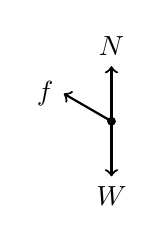
\begin{tikzpicture}[scale=.7]
      \fill[black](0,0) circle(.08);
      \draw[thick,->](0,0)--(0,1)node[pos=1,above]{$N$};
      \draw[thick,->](0,0)--(0,-1)node[pos=1,below]{$W$};
      \draw[thick,->,rotate=60](0,0)--(0,1)node[pos=1,left]{$f$};
    \end{tikzpicture}
    \item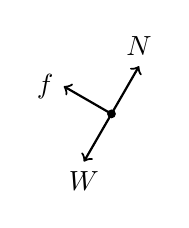
\begin{tikzpicture}[scale=.7]
        \fill[black](0,0) circle(.08);
        \draw[thick,->,rotate=-30](0,0)--(0,1)node[pos=1,above]{$N$};
        \draw[thick,->,rotate=-30](0,0)--(0,-1)node[pos=1,below]{$W$};
        \draw[thick,->,rotate=60](0,0)--(0,1)node[pos=1,left]{$f$};
    \end{tikzpicture}
    \item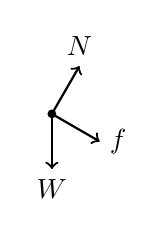
\begin{tikzpicture}[scale=.7]
      \fill[black](0,0) circle(.08);
      \draw[thick,->,rotate=-30](0,0)--(0,1)node[pos=1,above]{$N$};
      \draw[thick,->](0,0)--(0,-1)node[pos=1,below]{$W$};
      \draw[thick,->,rotate=60](0,0)--(0,-1)node[pos=1,right]{$f$};
    \end{tikzpicture}
    \item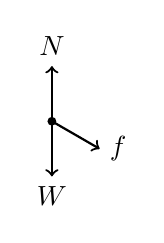
\begin{tikzpicture}[scale=.7]
      \fill[black](0,0) circle(.08);
      \draw[thick,->](0,0)--(0,1)node[pos=1,above]{$N$};
      \draw[thick,->](0,0)--(0,-1)node[pos=1,below]{$W$};
      \draw[thick,->,rotate=60](0,0)--(0,-1)node[pos=1,right]{$f$};
    \end{tikzpicture}
    \item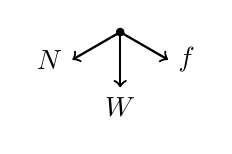
\begin{tikzpicture}[scale=.7]
      \fill[black](0,0) circle(.08);
      \draw[thick,->,rotate=120](0,0)--(0,1)node[pos=1,left]{$N$};
      \draw[thick,->](0,0)--(0,-1)node[pos=1,below]{$W$};
      \draw[thick,->,rotate=60](0,0)--(0,-1)node[pos=1,right]{$f$};
    \end{tikzpicture}
    \end{enumerate}

  \item The magnitude of the frictional force $f$ between the block and the
    plane is most nearly
    \begin{enumerate}[noitemsep,topsep=0pt,leftmargin=18pt,label=(\Alph*)]
    \item\SI{1}{\newton}
    \item\SI{2}{\newton}
    \item\SI{3}{\newton}
    \item\SI{4}{\newton}
    \item\SI{5}{\newton}
    \end{enumerate}
    \columnbreak
    
  \item A force gives an \SI{8}{\kilo\gram} mass an acceleration of
    \SI{3}{m/s^2}. The same force will give a \SI{12}{\kilo\gram} mass an
    acceleration of
    \begin{enumerate}[noitemsep,topsep=0pt,leftmargin=18pt,label=(\Alph*)]
    \item\SI{1}{\metre\per\second^2}
    \item\SI{2}{\metre\per\second^2}
    \item\SI{3}{\metre\per\second^2}
    \item\SI{4}{\metre\per\second^2}
    \item\SI{6}{\metre\per\second^2}
    \end{enumerate}

  \item Two blocks are pulled by a force of magnitude $F$ along a level surface
    with negligible friction as shown. The tension in the string between the
    blocks is
    \begin{center}
      \vspace{-.1in}\pic{.3}{connect2.png}
    \end{center}
    \begin{enumerate}[noitemsep,topsep=0pt,leftmargin=18pt,label=(\Alph*)]
    \item $\displaystyle\frac{1}{4}F$
    \item $\displaystyle\frac{1}{2}F$
    \item $\displaystyle\frac{1}{3}F$
    \item $F$
    \item $2F$
    \end{enumerate}
    
  \item A force of magnitude $F$ pulls up at an angle $\theta$ to the
    horizontal on a block of mass $m$. The mass remains in contact with the
    level floor and the coefficient of friction between the block and the floor
    is $\mu$. The frictional force between the floor and the block is
    \begin{center}
      \pic{.22}{angle1.png}
    \end{center}
    \begin{enumerate}[noitemsep,topsep=0pt,leftmargin=18pt,label=(\Alph*)]
    \item$\mu mg$
    \item$\mu (mg-F\sin\theta)$
    \item$\mu (mg+F\sin\theta)$
    \item$\mu (mg-F\cos\theta)$
    \item$\mu (mg+F\cos\theta)$
    \end{enumerate}

  %\item A block weighing \SI{60}{\newton} hangs from three ropes as shown.
  %  Which of the following statements is true?
  %  \begin{center}
  %    \vspace{-.1in}\pic{.3}{hanging.png}
  %  \end{center}
  %  \begin{enumerate}[noitemsep,topsep=0pt,leftmargin=18pt,label=(\Alph*)]    
  %  \item Each rope has a tension of \SI{60}{\newton}.
  %  \item The tension in each rope is higher in the lower part than in the
  %    upper part of the rope.
  %  \item The tension in each rope is higher in the upper part than in the
  %    lower part of the rope.
  %  \item The rope in the center has a higher tension than the othertwo ropes.
  %  \item Each rope has a tension of \SI{20}{\newton}.
  %  \end{enumerate}
    \columnbreak
    
  \item A stone falls through the air toward the Earth's surface. The resistive
    force the air applies to the stone as it falls is given by the equation
    $F=cv$, where $c$ is a positive constant and $v$ is the speed of the stone.
    The acceleration of the ball is given by the equation
    \begin{enumerate}[noitemsep,topsep=0pt,leftmargin=18pt,label=(\Alph*)]
    \item $c-g$
    \item $gcv/m$
    \item $g+cv$
    \item $g-cv/m$
    \item $cv/m$
    \end{enumerate}
    
  \item A block of mass $4m$ can move without friction on a horizontal surface.
    Another block of mass $m$ is attached to the larger block by a string that
    is passed over a light pulley. The acceleration of the system is

    \vspace{-.2in}\cpic{.2}{atwood1.png}
    \begin{enumerate}[noitemsep,topsep=0pt,leftmargin=18pt,label=(\Alph*)]
    \item $\displaystyle\frac{1}{5} g$
    \item $\displaystyle\frac{1}{2} g$
    \item $\displaystyle\frac{2}{3} g$
    \item $g$
    \item $5g$
    \end{enumerate}

  \item The block of mass $4m$ in the previous question now moves on a rough
    surface. The frictional force between the surface and the larger block is
    equal to $\frac{1}{2}mg$. The acceleration of the system is now
    \begin{enumerate}[noitemsep,topsep=0pt,leftmargin=18pt,label=(\Alph*)]
    \item $\frac{1}{16}g$
    \item $\frac{1}{10}g$
    \item $\frac{1}{4}g$
    \item $\frac{1}{2}g$
    \item $g$
    \end{enumerate}
  \end{enumerate}
  \columnbreak
  
  \textbf{Questions 30-31}

  A \SI{10}{\newton} block sits atop an inclined plane in the shape of a
  right triangle of sides \SI{3}{\metre}, \SI{4}{\metre}, and \SI{5}{\metre},
  as shown. The block is allowed to slide down the plane with negligible
  friction.
  \vspace{-.2in}\cpic{.2}{ramp3.png}
  
  \begin{enumerate}[resume,leftmargin=18pt]
  \item The acceleration of the block is most nearly
    \begin{enumerate}[noitemsep,topsep=0pt,leftmargin=18pt,label=(\Alph*)]
    \item\SI{2}{m/s^2}
    \item\SI{4}{m/s^2}
    \item\SI{6}{m/s^2}
    \item\SI{10}{m/s^2}
    \item\SI{12}{m/s^2}
    \end{enumerate}

  \item The normal force exerted on the block by the plane is most nearly
    \begin{enumerate}[noitemsep,topsep=0pt,leftmargin=18pt,label=(\Alph*)]
    \item\SI{2}{\newton}
    \item\SI{4}{\newton}
    \item\SI{6}{\newton}
    \item\SI{8}{\newton}
    \item\SI{10}{\newton}
    \end{enumerate}
    
  %\item A projectile is launched at an angle and follows a parabolic path near
  %  the Earth's surface. Which of the following best indicates the net force
  %  acting on the projectile at the top of its path, if any?


  \item Three strings are attached to a ring in the center of a force table. The
    top view of the force table is shown. For the ring to remain in the
    center of the table, which of the following must be true?
    \cpic{.18}{3strings.png}
    \begin{enumerate}[noitemsep,topsep=0pt,leftmargin=18pt,label=(\Alph*)]
    \item The vector sum of the three forces must equal zero.
    \item The lengths of the strings must be equal.
    \item The strings must form an angle of \ang{90} relative to each other.
    \item The magnitudes of two of the tensions in the strings must equal the
      tension in the third string.
    \item The tension in each string must be equal to each other.
    \end{enumerate}
  \end{enumerate}
  
  \textbf{Questions 33-34}

  The position of a \SI{2}{\kilo\gram} object is described by the equation
  $x=2t^2-3t^3$, where $x$ is in meters and $t$ is in seconds.
  \begin{enumerate}[resume,leftmargin=18pt]
  \item The net force acting on the object at a time of \SI{1}{s} is
    \begin{enumerate}[noitemsep,topsep=0pt,leftmargin=18pt,label=(\Alph*)]
    \item\SI{-4}{\newton}
    \item\SI{-8}{\newton}
    \item\SI{-14}{\newton}
    \item\SI{-20}{\newton}
    \item\SI{-24}{\newton}
    \end{enumerate}

  \item The net force acting on the object is positive from $t=0$ until a time
    of
    \begin{enumerate}[noitemsep,topsep=0pt,leftmargin=18pt,label=(\Alph*)]
    \item\SI{.11}{\second}
    \item\SI{.22}{\second}
    \item\SI{.44}{\second}
    \item\SI{.67}{\second}
    \item\SI{1.}{\second}
    \end{enumerate}
  \end{enumerate}
  
  \textbf{Questions 35-36}
  
  A particle of mass \SI{.5}{\kilo\gram} moves in two dimensions
  according to the velocity equation
  $\mb{v}=4t^2\bm{\hat{\imath}} + 6t^4 \bm{\hat{\jmath}}$, where speed is in
  \si{m/s} and time is in \si{\second}.

  \begin{enumerate}[resume,leftmargin=18pt]
  \item The acceleration of the particle at time $t=\SI{1}{s}$ in \si{m/s^2} is
    \begin{enumerate}[noitemsep,topsep=0pt,leftmargin=18pt,label=(\Alph*)]
    \item $a=8\bm{\hat{\imath}} + 24\bm{\hat{\jmath}}$
    \item $a=24\bm{\hat{\imath}} + 8\bm{\hat{\jmath}}$
    \item $a=8\bm{\hat{\imath}} + 48\bm{\hat{\jmath}}$
    \item $a=4\bm{\hat{\imath}} + 6\bm{\hat{\jmath}}$
    \item $a=2\bm{\hat{\imath}} + 8\bm{\hat{\jmath}}$
    \end{enumerate}

  \item The magnitude of the net force acting on the particle at a time of
    \SI{2}{s} is most nearly
    \begin{enumerate}[noitemsep,topsep=0pt,leftmargin=18pt,label=(\Alph*)]
    \item\SI{36}{\newton}
    \item\SI{64}{\newton}
    \item\SI{72}{\newton}
    \item\SI{84}{\newton}
    \item\SI{104}{\newton}
    \end{enumerate}
    \columnbreak
    
  \item A constant force acts on a particle in such a way that the direction of
    the force is always perpendicular to its velocity. Which of the
    following is true of the particle's motion?
    \begin{enumerate}[noitemsep,topsep=0pt,leftmargin=18pt,label=(\Alph*)]
    \item The acceleration of the particle is increasing
    \item The acceleration of the particle is decreasing.
    \item The speed of the particle is increasing.
    \item The speed of the particle is constant.
    \item The speed of the particle is decreasing.
    \end{enumerate}

  %\item A coffee filter is released from rest at a height of $3$ meters above
  %  the floor. Which of the following graphs best describes the speed of the
  %  falling coffee filter as a function of time?
  %  \begin{enumerate}[noitemsep,topsep=0pt,leftmargin=18pt,label=(\Alph*)]
  %  \item
  %  \item
  %  \item
  %  \item
  %  \item
  %  \end{enumerate}
  \end{enumerate}
  \columnbreak
  
  \textbf{Questions 38-39}

  A block of mass \SI{2}{\kilo\gram} rests on top of a larger block of mass
  \SI{4}{\kilo\gram}. The larger block slides without friction on a table, but
  the surface between the two blocks is not frictionless. The coefficient of
  friction between the two blocks is $0.2$. A horizontal force $\mb{F}$ is
  applied to the \SI{4}{\kilo\gram} mass.
  \cpic{.25}{stacked.png}
  \begin{enumerate}[resume,leftmargin=18pt]
  \item What is the maximum force that can be applied such that there is no
    relative motion between the two blocks?
    \begin{enumerate}[noitemsep,topsep=0pt,leftmargin=18pt,label=(\Alph*)]
    \item zero
    \item \SI{1}{\newton}
    \item \SI{2}{\newton}
    \item \SI{4}{\newton}
    \item \SI{12}{\newton}
    \end{enumerate}

  \item What is the acceleration of the \SI{2}{\kilo\gram} block relative to the
    \SI{4}{\kilo\gram} block if a force is applied to the \SI{4}{\kilo\gram}
    block that causes the \SI{4}{\kilo\gram} block to accelerate at
    \SI{3}{m/s^2} to the right?
    \begin{enumerate}[noitemsep,topsep=0pt,leftmargin=18pt,label=(\Alph*)]
    \item\SI{1}{m/s^2} to the right
    \item\SI{1}{m/s^2} to the left
    \item\SI{2}{m/s^2} to the right
    \item\SI{2}{m/s^2} to the left
    \item zero
    \end{enumerate}
  \end{enumerate}
\end{multicols}

\newpage
\begin{center}
  {\Large
    \textbf{AP\textsuperscript{\textregistered} Physics 1 \& C: Dynamics\\
      Student Answer Sheet for Multiple-Choice Section}
  }
  
  \begin{minipage}[t]{.3\textwidth}
    \vspace{.2in}
    \bgroup
    \begin{tabular}{>{\centering}m{1.3cm} >{\centering}m{1.7cm}}
      No. & Answer
    \end{tabular}\\
    \def\arraystretch{1.5}
    \begin{tabular}{|>{\centering}m{1.3cm}|>{\centering}m{1.7cm}|}
      \hline
      1 & \\ \hline
      2 & \\ \hline
      3 & \\ \hline
      4 & \\ \hline
      5 & \\ \hline
      6 & \\ \hline
      7 & \\ \hline
      8 & \\ \hline
      9 & \\ \hline
      10 & \\ \hline
      11 & \\ \hline
      12 & \\ \hline
      13 & \\ \hline
      14 & \\ \hline
      15 & \\ \hline
      16 & \\ \hline
      17 & \\ \hline
      18 & \\ \hline
      19 & \\ \hline
      20 & \\ \hline
      21 & \\ \hline
      22 & \\ \hline
      23 & \\ \hline
      24 & \\ \hline
      25 & \\ \hline
    \end{tabular}
    \egroup
  \end{minipage}
    \begin{minipage}[t]{.3\textwidth}
    \vspace{.2in}
    \bgroup
    \begin{tabular}{>{\centering}m{1.3cm} >{\centering}m{1.7cm}}
      No. & Answer
    \end{tabular}\\
    \def\arraystretch{1.5}
    \begin{tabular}{|>{\centering}m{1.3cm}|>{\centering}m{1.7cm}|}
      \hline
      26 & \\ \hline
      27 & \\ \hline
      28 & \\ \hline
      29 & \\ \hline
      30 & \\ \hline
      31 & \\ \hline
      32 & \\ \hline
      33 & \\ \hline
      34 & \\ \hline
      35 & \\ \hline
      36 & \\ \hline
      37 & \\ \hline
      38 & \\ \hline
      39 & \\ \hline
    \end{tabular}
    \egroup
  \end{minipage}
\end{center}
\newpage

\genfreetitle{1 \& C}{DYNAMICS}{2}

\genfreedirections{10}

\begin{enumerate}[leftmargin=15pt]

\item Three masses are connected by two strings as shown. One of the strings
  is passed over a pulley of negligible mass and friction. The pulley is
  attached to a stand that rests on a table. The smallest mass is $m$, the
  other two masses each have a mass of $2m$, and the mass of the stand is $4m$.
  \cpic{.2}{3masses.png}
  \begin{enumerate}[leftmargin=18pt]
  \item If the small mass $m$ is removed, the other two masses hang in
    equilibrium. Determine the normal force the table exerts on the stand
    when the system is in equilibrium.
    
  \item The small mass $m$ is once again hung below one of the masses of mass
    $2m$. Determine the acceleration of the system.

  \item Determine the tension in the string between the block of mass $2m$ and
    the attached block of mass m while the system is accelerating.

  \item While the system is accelerating, is the normal force exerted by the
    table on the stand greater than, equal to, or less than $8mg$? Justify your
    answer.
  \end{enumerate}
  \newpage
\item Two blocks weighing \SI{10}{\newton} each are connected by a light string
  that is passed over a light pulley. One of the blocks rests on an inclined
  plane at an angle of \ang{37} to the horizontal. The friction between the
  inclined plane and the block is such that the system remains at rest. The
  length of the ramp is \SI{5}{\metre}.
  \cpic{.3}{ramp4.png}
  \begin{enumerate}[leftmargin=18pt]
  \item Determine the tension in the string while the system is at rest.
  \item Determine the frictional force between the block and the inclined plane
    while the system is at rest.
  \item If the string is suddenly cut, what is the speed of the block when it
    reaches the bottom of the plane?
  \end{enumerate}
\end{enumerate}

\end{document}
